\documentclass[fleqn,a4paper,11pt]{article}
\title{Noughts and Crosses}
\author{Izaak van Dongen}

\usepackage{mysty}

\begin{document}
    \maketitle\thispagestyle{empty} % no page number under title
    \tableofcontents
    \listoflistings

    \section{Introduction}

    This is a set of programs that enable a user to play noughts and crosses
    ``locally with a friend'' (themselves), or to play against a computer, or
    even to watch the computer desperately trying to win against itself. It also
    supports arbitrarily sized boards, and probably several cases of overly
    optimised approaches to problems like the detection of a winning condition
    on a board.

    Internally, the board is represented as one-dimensional array (arraylist) of
    any of \mintinline{python}|{None, True, False}|, corresponding to
    \(\{\text{Empty, Crosses, Noughts}\}\). The single dimensionality is actually
    pretty natural, as a noughts and crosses board is not fundamentally a list
    of lists, but a set of tiles with some subsets considered to be ``in a
    row''. The board is enumerated from the top-left tile, left-to-right,
    top-to-bottom. When x-y indexing is used, the co-ordinate \((x,y)\)
    corresponds to the index \(3y+x\). This has a couple of nice properties which
    will come up later.

    Minmax is implemented by a single ``optimise'' function that recursively
    searches the tree, with several specialisations over general minmax. These
    include for example not having to keep maximising after encounting a win, as
    the evaluation heuristic is known to only be able to evaluate the board as
    \(\{\text{win}, \text{lose}, \text{draw}\}\).

    The tests for winning conditions are implemented in listing
    \ref{lst:checkingpy}. They work by instantiating a single list of indices
    for each subset considered a ``row'', and then creating an array indexed by
    board indices of lists of these subsets, where the subsets stored at a board
    index represent all the rows that tile is a part of.

    Further explanation of implementation details may be included in docstrings
    in the source.

    I decided to develop in Python as I had some quite ambitious ideas about the
    algorithm, which I thought would be easier to express by using the more
    functional side of Python. Python is also nicely expressive, which makes it
    easier to develop without getting bogged down in syntax. Similarly, I wrote
    a command-line program because it doesn't involve using Lazarus.

    \section{Implementation}

    Listing \ref{lst:basepy} has some boilerplate classes that are shared
    throughought, to give some abstract representation of the game.

\begin{longlisting}
\inputminted{python}{../src/base.py}
\caption{\texttt{base.py}: Some shared base classes}
\label{lst:basepy}
\end{longlisting}

    Listing \ref{lst:checkingpy} implements all of the ``checking'' - this is
    mostly the generation of rows and groups, and then some simple list
    comprehensions and generator expressions to evaluate a board using these.

    The subsets are represented as Python \texttt{range}s. This is possible as
    each row is a linear succession of indices in this linearisation of the
    board. These ranges are implemented very efficiently, using only integer
    arithmetic to generate intermediate range values or to determine membership.

    Because these groups are used often, they are stored in a registry and
    generated when needed. This is all handled by the module itself, so a user
    only needs to call \texttt{get\_groups}.

\begin{longlisting}
\inputminted{python}{../src/checking.py}
\caption{\texttt{checking.py}: Implementation of minimax}
\label{lst:checkingpy}
\end{longlisting}

    When the module is run directly, it dumps all of the groups for a given
    board size. Listing \ref{lst:checkingout} has a sample of this behaviour
    (and also demonstrates the nice board formatting).

\begin{longlisting}
\begin{minted}{text}
% python checking.py 3
0 [range(0, 3), range(0, 9, 3), range(0, 9, 4)]
   0   1   2
 0 M | G | G 
  ---+---+---
 1   |   |   
  ---+---+---
 2   |   |   

   0   1   2
 0 M |   |   
  ---+---+---
 1 G |   |   
  ---+---+---
 2 G |   |   

   0   1   2
 0 M |   |   
  ---+---+---
 1   | G |   
  ---+---+---
 2   |   | G 

1 [range(0, 3), range(1, 10, 3)]
   0   1   2
 0 G | M | G 
  ---+---+---
 1   |   |   
  ---+---+---
 2   |   |   

   0   1   2
 0   | M |   
  ---+---+---
 1   | G |   
  ---+---+---
 2   | G |   

2 [range(0, 3), range(2, 11, 3), range(2, 7, 2)]
   0   1   2
 0 G | G | M 
  ---+---+---
 1   |   |   
  ---+---+---
 2   |   |   

   0   1   2
 0   |   | M 
  ---+---+---
 1   |   | G 
  ---+---+---
 2   |   | G 

   0   1   2
 0   |   | M 
  ---+---+---
 1   | G |   
  ---+---+---
 2 G |   |   
\end{minted}
\caption{Output of \texttt{checking.py}}\label{lst:checkingout}
\end{longlisting}

    Listing \ref{lst:computerpy} shows the implementation of minimax with all
    previously described bells and whistles. When called directly, it can
    demonstrate its approach to a particular board state, shown in listing
    \ref{lst:computerout}. My favourite part of this program is the generator
    \texttt{generate\_moves}.

\begin{longlisting}
\inputminted{python}{../src/computer.py}
\caption{\texttt{computer.py}: Implementation of minimax}
\label{lst:computerpy}
\end{longlisting}

\begin{longlisting}
\begin{minted}{text}
% python computer.py -b "x__ _o_ o_x"   
[True, None, None, None, False, None, False, None, True] 3
   0   1   2
 0 X |   |   
  ---+---+---
 1   | O |   
  ---+---+---
 2 O |   | X 

    Examining as O 5:
        0   1   2
      0 X | X |   
       ---+---+---
      1   | O |   
       ---+---+---
      2 O |   | X 
       Examining as X 6:
           0   1   2
         0 X | X | O 
          ---+---+---
         1   | O |   
          ---+---+---
         2 O |   | X 
       State here: State.O_WIN
    Examining as O 5:
        0   1   2
      0 X |   | X 
       ---+---+---
      1   | O |   
       ---+---+---
      2 O |   | X 
       Examining as X 6:
           0   1   2
         0 X | O | X 
          ---+---+---
         1   | O |   
          ---+---+---
         2 O |   | X 
          Examining as O 7:
              0   1   2
            0 X | O | X 
             ---+---+---
            1 X | O |   
             ---+---+---
            2 O |   | X 
             Examining as X 8:
                 0   1   2
               0 X | O | X 
                ---+---+---
               1 X | O | O 
                ---+---+---
               2 O |   | X 
                Examining as O 9:
                    0   1   2
                  0 X | O | X 
                   ---+---+---
                  1 X | O | O 
                   ---+---+---
                  2 O | X | X 
                Draw here
             Examining as X 8:
                 0   1   2
               0 X | O | X 
                ---+---+---
               1 X | O |   
                ---+---+---
               2 O | O | X 
             State here: State.O_WIN
          Examining as O 7:
              0   1   2
            0 X | O | X 
             ---+---+---
            1   | O | X 
             ---+---+---
            2 O |   | X 
          State here: State.X_WIN
       Examining as X 6:
           0   1   2
         0 X |   | X 
          ---+---+---
         1 O | O |   
          ---+---+---
         2 O |   | X 
          Examining as O 7:
              0   1   2
            0 X | X | X 
             ---+---+---
            1 O | O |   
             ---+---+---
            2 O |   | X 
          State here: State.X_WIN
       Examining as X 6:
           0   1   2
         0 X |   | X 
          ---+---+---
         1   | O | O 
          ---+---+---
         2 O |   | X 
          Examining as O 7:
              0   1   2
            0 X | X | X 
             ---+---+---
            1   | O | O 
             ---+---+---
            2 O |   | X 
          State here: State.X_WIN
       Examining as X 6:
           0   1   2
         0 X |   | X 
          ---+---+---
         1   | O |   
          ---+---+---
         2 O | O | X 
          Examining as O 7:
              0   1   2
            0 X | X | X 
             ---+---+---
            1   | O |   
             ---+---+---
            2 O | O | X 
          State here: State.X_WIN
Win incoming
Computer plays at (2, 0)
   0   1   2
 0 X |   | X 
  ---+---+---
 1   | O |   
  ---+---+---
 2 O |   | X 
\end{minted}
\caption{Output of \texttt{computer.py}}\label{lst:computerout}
\end{longlisting}

    Listing \ref{lst:formattingpy} contains the code that formats boards as seen
    in previous listings (such as \ref{lst:computerout} and
    \ref{lst:checkingout}). It works by generating a ``template'' string, which
    is a string that is in a format that can be string-interpolated by
    \texttt{str.format}. It uses a similar registry principle to listing
    \ref{lst:checkingpy}.

    It makes most judicious use of Python various inline iteration capability,
    relegating the template generation to a single lexical line of code.

    It can also demo its functionality when run directly, as shown in listing
    \ref{lst:formattingout}

\begin{longlisting}
\inputminted{python}{../src/formatting.py}
\caption{\texttt{formatting.py}: Formatting internal board arrays as strings}
\label{lst:formattingpy}
\end{longlisting}

\begin{longlisting}
\begin{minted}{text}
% python formatting.py 5
5x5 template:
   0   1   2   3   4
 0 {} | {} | {} | {} | {}
  ---+---+---+---+---
 1 {} | {} | {} | {} | {}
  ---+---+---+---+---
 2 {} | {} | {} | {} | {}
  ---+---+---+---+---
 3 {} | {} | {} | {} | {}
  ---+---+---+---+---
 4 {} | {} | {} | {} | {}

random 5x5 board:
   0   1   2   3   4
 0 X |   | X | X | X
  ---+---+---+---+---
 1 X | X | O | X |
  ---+---+---+---+---
 2   | X | X | O | O
  ---+---+---+---+---
 3 X |   |   |   |
  ---+---+---+---+---
 4 O | X | O | X | X
\end{minted}
\caption{Output of \texttt{formatting.py}}\label{lst:formattingout}
\end{longlisting}

    Listing \ref{lst:interfacepy} deals with some of the really dull stuff, like
    getting user input.

\begin{longlisting}
\inputminted{python}{../src/interface.py}
\caption{\texttt{interface.py}: Dealing with user input}
\label{lst:interfacepy}
\end{longlisting}

    Listing \ref{lst:playpy} ties it all together, providing a pretty sophisticated
    interface through command-line arguments (see the \texttt{get\_args}
    function). It allows you to play against yourself, the computer, or even
    just for you to watch the computer instantly force itself into a draw, if
    that's your thing.

    The only other application of the \texttt{--battle} mode is to change the
    size of the board to anything more than 3, and watch your CPU melt. This is
    due to the size of the search tree growing with \(\BigO(2^{(n^2)})\), which,
    however, nicely implemented your tree search is, is a bit of a party-pooper.

    A sample of play is provided in listing \ref{lst:playout}

\begin{longlisting}
\inputminted{python}{../src/play.py}
\caption{\texttt{play.py}: Bringing it all together to play the game}
\label{lst:playpy}
\end{longlisting}

\begin{longlisting}
\begin{minted}{text}
Computer plays at (0, 0)
   0   1   2
 0 X |   |   
  ---+---+---
 1   |   |   
  ---+---+---
 2   |   |   

   0   1   2
 0 X |   |   
  ---+---+---
 1   |   |   
  ---+---+---
 2   |   |   

You are playing as noughts
Enter the position you want to play in > 1 0
Computer plays at (0, 1)
   0   1   2
 0 X | O |   
  ---+---+---
 1 X |   |   
  ---+---+---
 2   |   |   

   0   1   2
 0 X | O |   
  ---+---+---
 1 X |   |   
  ---+---+---
 2   |   |   

You are playing as noughts
Enter the position you want to play in > 0 2
Computer plays at (1, 1)
   0   1   2
 0 X | O |   
  ---+---+---
 1 X | X |   
  ---+---+---
 2 O |   |   

   0   1   2
 0 X | O |   
  ---+---+---
 1 X | X |   
  ---+---+---
 2 O |   |   

You are playing as noughts
Enter the position you want to play in > 2 2
Computer plays at (2, 1)
   0   1   2
 0 X | O |   
  ---+---+---
 1 X | X | X 
  ---+---+---
 2 O |   | O 

Win: I'm sorry, Dave. I'm afraid I can't do that.
\end{minted}
\caption{Output of \texttt{play.py}}\label{lst:playout}
\end{longlisting}

    \section{Interface}

    Also provided is an elegant (bare) interface written in Processing, for ease
    of translation of Python and graphics primitives. It reuses most of the same
    code, stripping out parts that print, and involved a slight rewrite of
    \texttt{generate\_moves}, due to Python 2's alternative handling of finally
    clauses. A diff of the library code adapted for graphical Python 2 is shown
    in listing \ref{lst:procdiff}.

    This was written with very little time to spare, so excuse my slightly
    square crosses and sloppy code here.

\begin{longlisting}
\begin{minted}{diff}
$ for i in *.py; do echo $i; diff $i src/$i; done
base.py
4a5,6
> from enum import Enum
>
23c25
< class State(object):
---
> class State(Enum):
checking.py
7a8
> from formatting import get_board_template
81a83
>             print(board_temp.format(*dft), end="\n\n")
computer.py
5a6,8
> from textwrap import indent
> from traceback import extract_stack
>
7a11
> from formatting import print_board, strfboard, syms
72a77,80
>     verbose and print(indent("Examining as {} {}:\n{}"
>                          .format(syms[crosses_playing], depth,
>                             indent(strfboard(board, n), ' ')),
>                       ' ' * len(extract_stack())))
74a83,84
>         verbose and print(indent("State here: {}"
>                   .format(state), " " * len(extract_stack())))
76a87
>         verbose and print(indent("Draw here", " " * len(extract_stack())))
82c93
<                    for move, board in generate_moves(board[:], crosses_playing)),
---
>                    for move, board in generate_moves(board, crosses_playing)),
103a115
>             verbose and print("Win incoming")
105a118
>             verbose and print("Draw forcable")
117a131,132
>     print("Computer plays at ({}, {})".format(move % n, move // n))
>     print_board(board, n)
interface.py
5a6
> from formatting import print_board, syms
\end{minted}
\caption{Diff of processing code vs core src}\label{lst:procdiff}
\end{longlisting}

    The drawing code is shown in listing \ref{lst:procpy}

\begin{longlisting}
\inputminted{python}{../noughtsandcrosses.pyde}
\caption{Processing code to handle user interaction and drawing of board}\label{lst:procpy}
\end{longlisting}

    The game's modern design is shown in figure \ref{fig:proc}

\begin{figure}[H]
\begin{center}
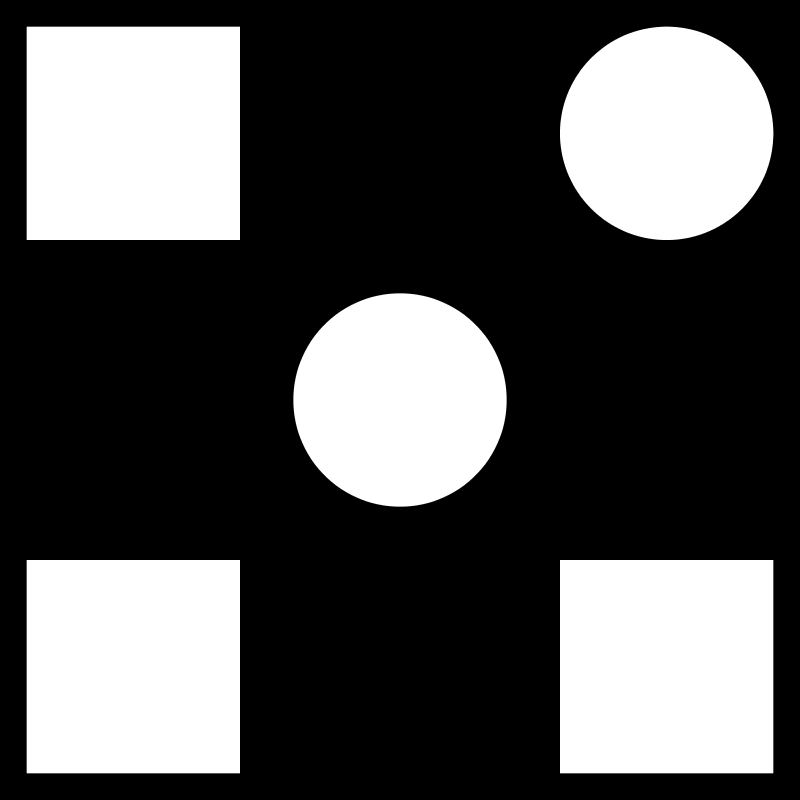
\includegraphics[width=0.5\textwidth]{../win_screenshot_20180712_110639.png}
\caption{The new way to play noughts and crosses}\label{fig:proc}
\end{center}
\end{figure}

    \section{Source}

    The full project in its directory structure, including this document (as a
    full-colour PDF and \TeX{} file), can be found at
    \url{https://github.com/goedel-gang/noughtsandcrosses}.

\end{document}
